\section{Results}
\label{section:results}
The objective of this study is to evaluate the effectiveness and robustness of Bayesian SegNet in marine semantic 
segmentation and to assess its predictive capability in novel environments. This evaluation is conducted through 
appropriate metrics. Initially, both Bayesian SegNet and SegNet were trained using the MaSTr1325 training dataset. 
After the models converged, their accuracy was validated against the MaSTr1325 validation dataset based on metrics. 
The performance of these two models was then compared to that of existing semantic segmentation architectures, 
highlighting the Bayesian approach's ability to remove noisy data and improve accuracy. Additionally, this study 
captures both aleatoric and epistemic uncertainty, providing qualitative analysis of these aspects. Finally, the 
Bayesian and non-Bayesian models trained on the MaSTr1325 dataset were used to predict images from the OASIs dataset, 
demonstrating that Bayesian models offer better inference capabilities in novel scenarios. 

\subsection{Model Training and Performance Evaluation}
\label{section:MTPE}
Before training the model, the MaSTr1325 dataset needs to be partitioned for different uses. The dataset was randomly 
split into a 7:2:1 ratio, with 927 images allocated for training, 266 for validation, and 132 for testing, each 
accompanied by corresponding annotations. The size of the training dataset ensures that the model can extract 
sufficient features \cite{MaSTr1325}, while this partitioning strategy helps mitigate the risk of overfitting. 
% figure
\begin{figure}[ht!]
    % subfig1
    \centering
    \begin{subfigure}[b]{\textwidth}
        \centering
        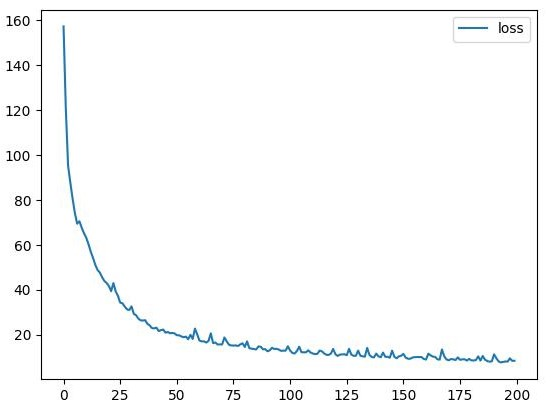
\includegraphics[width=0.32\textwidth]{figures/MaSTr1325/trainloss-nonebayes.jpg}
        \caption{}
        \label{fig:nbs-mastr1325-tl}
    \end{subfigure}
    % subfig2
    \centering
    \begin{subfigure}[b]{0.9\textwidth}
        \centering
        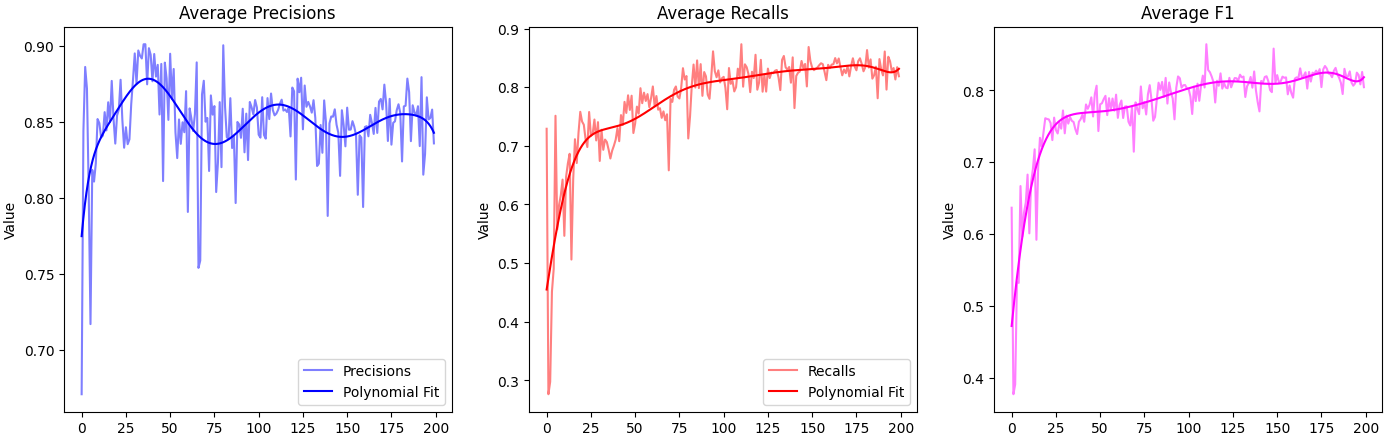
\includegraphics[width=\textwidth]{figures/MaSTr1325/validation-nonebayes.png}
        \caption{}
        \label{fig:nbs-mastr1325-val}
    \end{subfigure}
    \caption{Performance of non-Bayesian SegNet on the MaSTr1325 dataset: 
    (a) Training loss curve using Cross-Entropy Loss, (b) Evaluation metrics curves.}
    \label{fig:nbs-mastr1325-perf}
\end{figure}

During the training of non-Bayesian SegNet using the training dataset from MaSTr1325, the Cross-Entropy Loss for 
each image is computed and accumulated for every iteration within each epoch to form the total training loss. This 
data is used to generate a training loss curve throughout the training process, which is shown in Fig.
\ref{fig:nbs-mastr1325-tl}. However, evaluating model convergence solely based on the training loss curve can be 
misleading, as excessive training may result in overfitting. To address this, the validation dataset is employed 
to help determine whether the model has converged or if overfitting has occurred. Evaluation metrics are used to 
generate an evaluation curve in Fig.\ref{fig:nbs-mastr1325-val}, providing additional insights into the model's 
performance.

For Bayesian SegNet, a distinct method is used for calculating training loss. Specifically, the negative 
log-likelihood loss (NLLL) is computed and averaged, while an accuracy curve for the predictions is also generated, 
as illustrated in Fig.\ref{fig:bs-mastr1325-tl}. Additionally, the validation dataset is used to evaluate the 
model's performance through appropriate evaluation metrics. The resulting metrics curves are depicted in Fig.
\ref{fig:bs-mastr1325-val}.
% figure
\begin{figure}[ht!]
    % subfig1
    \centering
    \begin{subfigure}[b]{\textwidth}
        \centering
        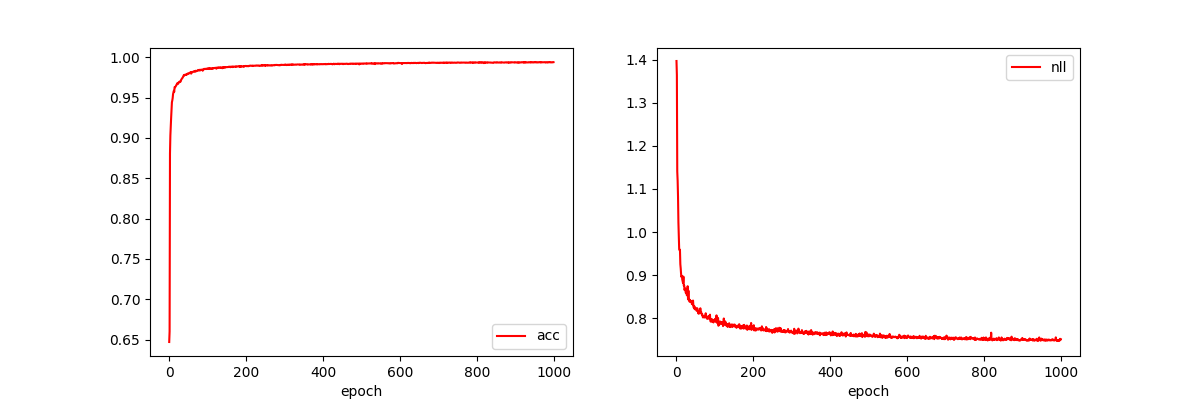
\includegraphics[width=0.75\textwidth]{figures/MaSTr1325/trainloss-bayes.png}
        \caption{}
        \label{fig:bs-mastr1325-tl}
    \end{subfigure}
    % subfig2
    \centering
    \begin{subfigure}[b]{\textwidth}
        \centering
        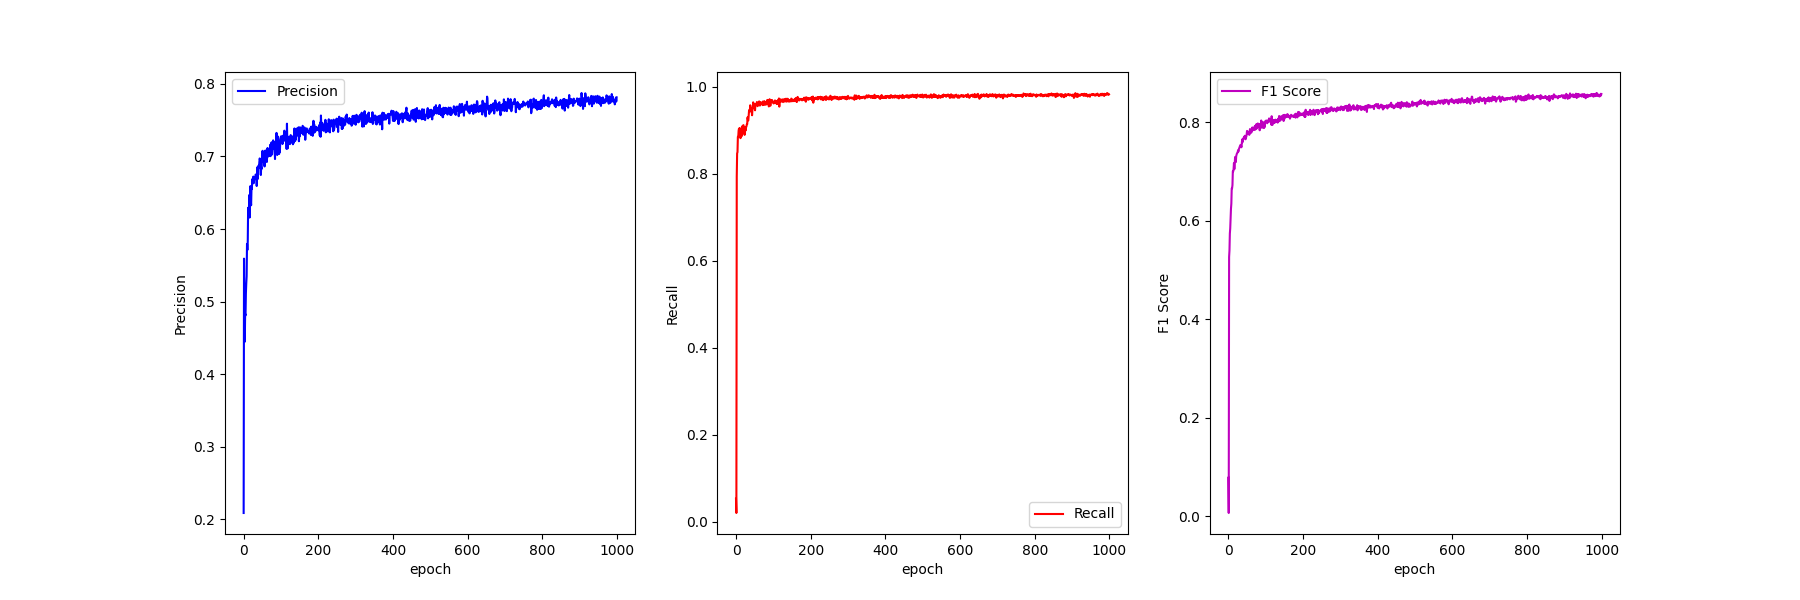
\includegraphics[height = 5cm, width=0.9\textwidth]{figures/MaSTr1325/validation-bayes.png}
        \caption{}
        \label{fig:bs-mastr1325-val}
    \end{subfigure}
    \caption{Performance of Bayesian SegNet on the MaSTr1325 dataset: 
    (a) Accuracy and training loss curves using NLLL, (b) Evaluation metrics curves.}
    \label{fig:bs-mastr1325-perf}
\end{figure}

In the calculation of evaluation metrics, a threshold of 0.2 is predominantly employed. This implies that if the 
softmax values for all classes are below 0.2, the pixel is labelled as "Unknown." This relatively low threshold 
encourages the algorithm to annotate regions with high uncertainty. However, the optimal threshold should be 
determined through empirical testing. Fig.\ref{fig:eval-threshold} presents the Precision ($\mathbf{Pr}$), 
Recall ($\mathbf{Re}$), and F1 score ($\mathbf{F1}$) for Bayesian and non-Bayesian SegNet models on the MaSTr1325 
validation dataset across varying thresholds.
% figure
\begin{figure}[ht!]
    \centering
    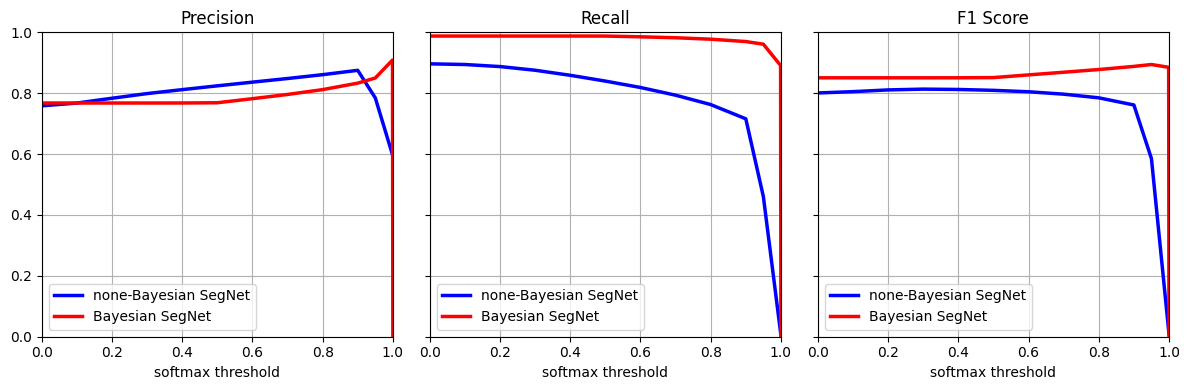
\includegraphics[width=0.9\textwidth]{figures/MaSTr1325/evaluation-threshold.png}
    \caption{,$\mathbf{Pr}$, $\mathbf{Re}$, and $\mathbf{F1}$ comparison for Bayesian and non-Bayesian SegNet models.}
    \label{fig:eval-threshold}
\end{figure}

The performance of the Bayesian SegNet can be compared with other networks trained on the MaSTr1325 dataset. In 
this context, it is compared with the Unet and PSPNet trained by Bovcon et al. \cite{MaSTr1325}, and the SegNet 
model trained in this study. The comparison is illustrated in Table \ref{tab:BS-vs-others}. It can be observed 
that accuracy has improved by 1.3\% compared to the non-Bayesian baseline, achieved by mitigating the impact of 
noisy data. Additionally, a significant reduction in False Negative rates (FNr) has led to a substantial increase 
in Recall. Compared to the other two architectures, the SegNet architecture has demonstrated its superiority in the 
field of maritime semantic segmentation, particularly through its outstanding $\mathbf{F1}$. Overall, the Bayesian 
SegNet architecture not only delivers highly accurate segmentation, but also effectively mitigates the impact of noise 
in the data on accuracy.
% table
\begin{table}[ht!]
    \centering
    \caption{Performance of Bayesian SegNet compared with other models.}
    \label{tab:BS-vs-others}
    \begin{tabular}{c|c|c|c}
    \textbf{Architecture}        & \textbf{Pr}(\%) & \textbf{Re}(\%) & \textbf{F1}(\%) \\ \hline
    Bayesian SegNet              & 81.2 & 97.8 & 87.8 \\ \hline 
    SegNet                       & 79.9 & 87.5 & 81.3 \\ \hline 
    PSPNet\cite{PSPNet}          & 82.1 & 50.8 & 62.8 \\ \hline
    U-Net\cite{UNet}             & 10.2 & 88.6 & 18.3 \\ \hline
    \end{tabular}
\end{table}

\subsection{Uncertainty Estimation}
\label{section:UE}
Fig.\ref{fig:bs-mastr1325-disp} shows segmentation and model uncertainty estmation from Bayesian SegNet on 
MaSTr1325 testing dataset. High epistemic uncertainty is often observed in instances where SegNet generates an 
incorrect class label. 
% figure
\begin{figure}[ht!]
    \centering
    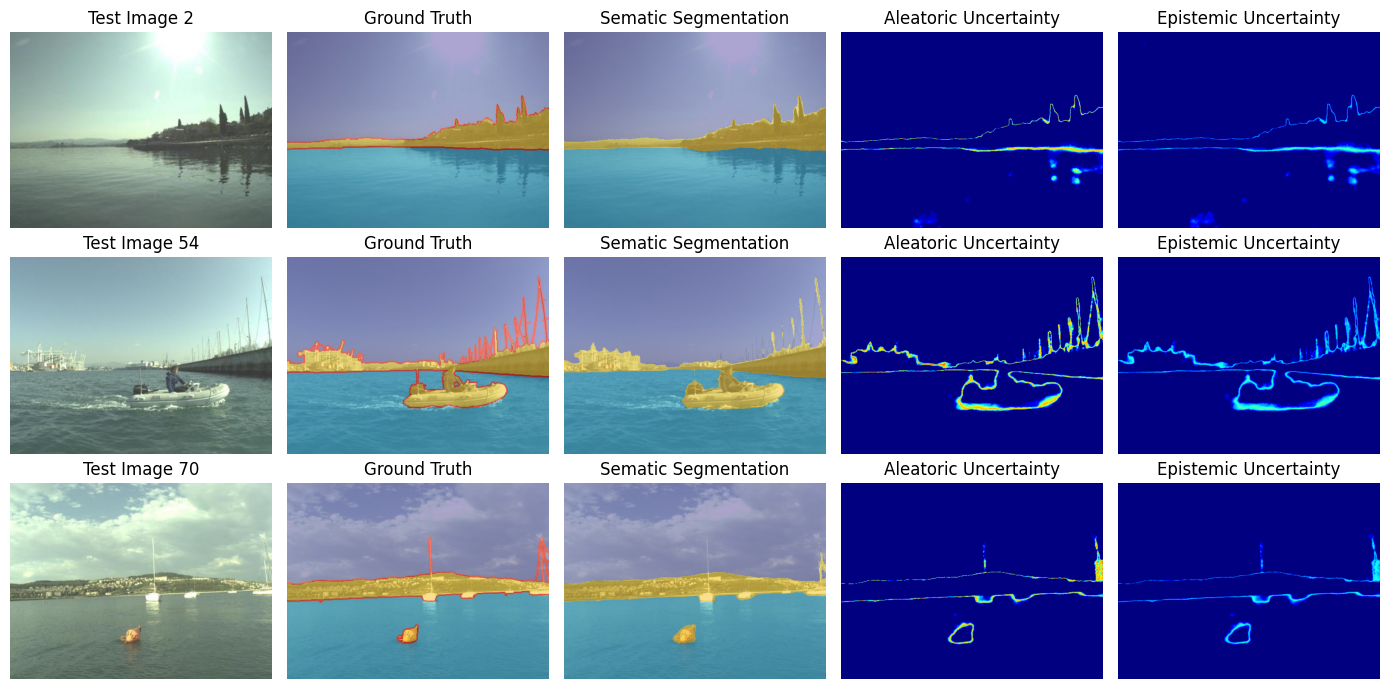
\includegraphics[width=0.9\textwidth]{figures/MaSTr1325/BayesianSegNet-panel.png}
    \caption{Bayesian SegNet on MaSTr1325 testing dataset.}
    \label{fig:bs-mastr1325-disp}
\end{figure} 

In Fig.\ref{fig:error1}, the uncertainty estimation results highlight two areas of notably high 
uncertainty, in addition to the object edges. These areas, marked with red boxes, are associated with distortions 
caused by reflections on the water surface. The area located at the bottom of the image exhibits distortion due 
to sunlight reflecting off the water. However, the point estimate of the model remains unaffected by this distortion 
and correctly assigns the class label. In contrast, the area on the right side of the image, presents some 
misclassifications, which are accompanied by a correspondingly high uncertainty estimation. In Fig.\ref{fig:error2}, 
a different misclassification scenario is observed, where the algorithm incorrectly identifies the wall as water. 
This misclassification may be due to the similar texture or colour patterns between the wall and the water surface, 
or due to poor lighting conditions that obscure the distinguishing features. However, these misclassified areas are 
accompanied by high levels of aleatoric and epistemic uncertainty. Overall, this approach provides a means of applying 
corrective measures in cases of misclassification, thereby enhancing the robustness of the USV perception module. 
% figure
\begin{figure}[ht!]
    % subfig1
    \centering
    \begin{subfigure}[h]{\textwidth}
        \centering
        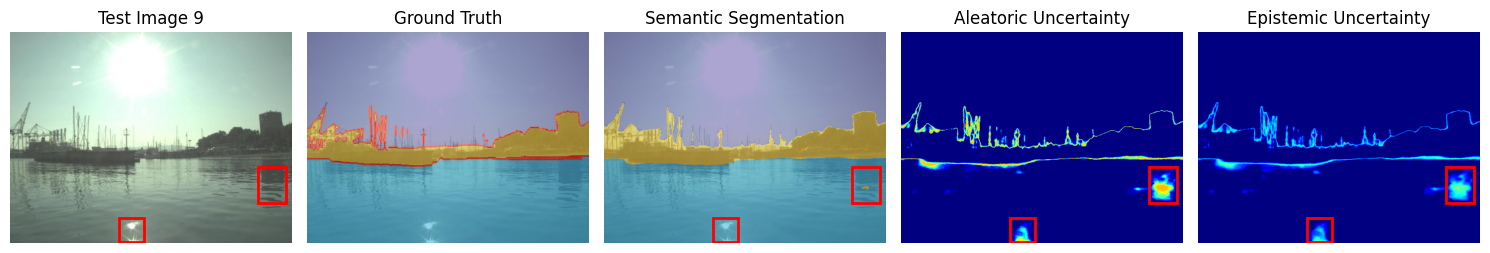
\includegraphics[width=0.9\textwidth]{figures/MaSTr1325/errorness1.png}
        \caption{}
        \label{fig:error1}
    \end{subfigure}
    % subfig2
    \centering
    \begin{subfigure}[h]{\textwidth}
        \centering
        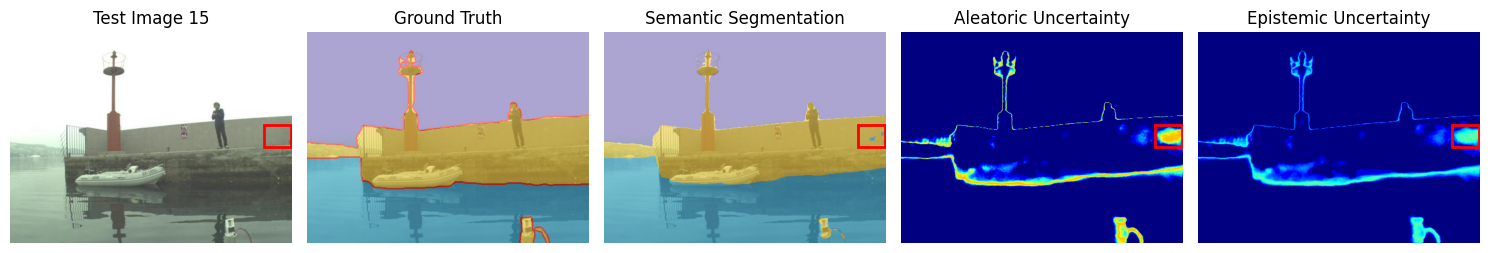
\includegraphics[width=0.9\textwidth]{figures/MaSTr1325/errorness2.png}
        \caption{}
        \label{fig:error2}
    \end{subfigure}
    \caption{Misclassifications with high uncertainty in different scenarios: 
    (a) Caused by water surface reflection, (b) Caused by wall texture similarity.}
    \label{fig:high-uncertainty}
\end{figure}

Additionally, to assess the potential of uncertainty in enhancing the performance of the perception module, the 
epistemic uncertainty threshold was set. Pixels with epistemic uncertainty exceeding this threshold were 
reclassified into class 4. This method was employed to determine whether integrating uncertainty can effectively 
improve the accuracy of semantic segmentation. In practical USV applications, the information regarding aleatoric 
and epistemic uncertainty should be handled by the path planning module, rather than simply excluding the 
segmentation results for regions with high uncertainty. 

As shown in Table \ref{tab:uncertainty-threshold}, it can be observed that as the threshold decreases, $\mathbf{Pr}$ 
and $\mathbf{F1}$ correspondingly increase, while $\mathbf{Re}$ decreases. Calculating the average number of True 
Positives ($\mathbf{TP_r}$), False Positives ($\mathbf{FP_r}$), and False Negatives ($\mathbf{FN_r}$)  reveals that 
as the threshold decreases, $\mathbf{FN_r}$ gradually increase, while $\mathbf{TP_r}$ and $\mathbf{FP_r}$ decreases. 
The table does not include thresholds of 0.6, 0.7, 0.8, and 0.9 because, in these cases, the maximum epistemic 
uncertainty is less than 0.5. Therefore, the values for thresholds between 0.5 and 1.0 are effectively the same.
% table
\begin{table}[ht!]
    \centering
    \caption{Performance of Bayesian SegNet compared with other models.}
    \label{tab:uncertainty-threshold}
    \begin{tabular}{c|c|c|c|c|c|c}
    \textbf{Epistemic Uncertainty Threshold} & $\mathbf{TP_r}$ &$\mathbf{FP_r}$ & $\mathbf{FN_r}$ & \textbf{Pr}(\%) & \textbf{Re}(\%) & \textbf{F1}(\%) \\ \hline
    1.00 & 14968.86 & 3301.41 & 457.17 & 76.78 & 98.78 & 85.06 \\ \hline 
    0.50 & 14968.86 & 3301.41 & 457.17 & 76.78 & 98.78 & 85.06 \\ \hline 
    0.40 & 14854.52 & 3045.23 & 571.51 & 78.05 & 98.36 & 85.98 \\ \hline
    0.30 & 14630.89 & 2462.62 & 795.14 & 81.08 & 97.50 & 87.69 \\ \hline
    0.20 & 14405.76 & 2009.39 & 1020.27 & 83.59 & 96.50 & 88.80 \\ \hline
    0.10 & 14085.67 & 1580.83 & 1340.36 & 86.21 & 94.85 & 89.56 \\ \hline 
    0.05 & 13858.67 & 1338.45 & 1567.36 & 87.72 & 93.52 & 89.74 \\ \hline 
    \end{tabular}
\end{table}

\subsection{Domain Transfer Evaluation}
\label{section:DTE}
To assess the generalization capabilities, Bayesian SegNet and non-Bayesian SegNet models trained on the 
MaSTr1325 dataset were evaluated using the OASIs dataset \cite{OASIs}. While many studies validate models trained 
on MaSTr1325 using the MODD2 dataset \cite{MODS,MODD2,WaSR}, this approach may have inherent limitations. Both 
datasets 
were collected with USVs in the Gulf of Koper, Slovenia \cite{MaSTr1325}, which might introduce subtle, shared 
features. Consequently, models trained on these datasets may inadvertently learn and rely on these latent 
characteristics, inaccurately representing them as features of the marine environment. To mitigate this issue, 
it is preferable to use marine environment datasets collected from different geographical regions for evaluation. 
Unlike the SMD dataset used by Borja Bovcon and Matej Kristan \cite{WaSR}, the OASIs dataset was chosen for its 
classification of data based on varied collection conditions, which supports a more comprehensive analysis. 

Fig.\ref{fig:bs-oasis-usv} shows segmentation and model uncertainty estimation from Bayesian SegNet 
on OASIs dataset. Each row of images corresponds to a different scenario. The first row (type 1) represents the 
Day-Time Environment, the second row (type 2) represents the Adverse Weather Environment, and the third row (type 3) 
indicates the Night-Time Environment. These categories are defined by the OASIs dataset.
% figure
\begin{figure}[ht!]
    \centering
    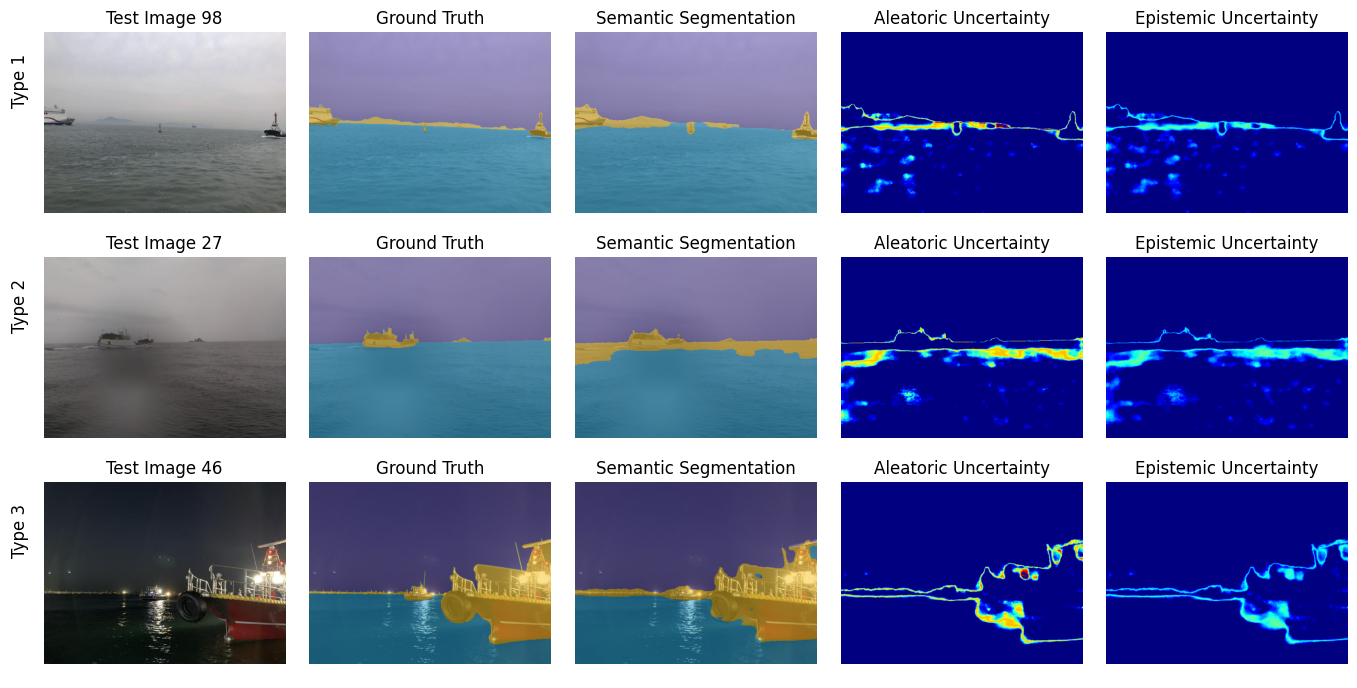
\includegraphics[width=0.9\textwidth]{figures/OASIs/BayesianSegNet-usv-panel.png}
    \caption{Bayesian SegNet performance evaluation on USV perspective.}
    \label{fig:bs-oasis-usv}
\end{figure} 

The performance evaluation on the MaSTr1325 validation dataset was conducted using the corresponding evaluation 
metrics. In the domain transfer evaluation, the same metrics were applied to assess the model's performance on the 
OASIs dataset. To facilitate a more detailed comparison, this study further subdivides the OASIs dataset. Since 
the OASIs dataset was captured from two perspectives, it is divided into the perspectives of USV and cargo ship. 
This study evaluates the model's performance across the three types in the OASIs dataset and their corresponding 
perspectives using the defined metrics. The results are compared with SegNet model trained on the MaSTr1325 dataset 
and evaluated on the SMD dataset \cite{WaSR}, which is illustrated in Table \ref{tab:DTEP}. 
% table
\begin{table}[ht!]
    \centering
    \caption{Evaluation on domain transfer performance.}
    \label{tab:DTEP}
    \begin{tabular}{c|c|c|c|c|c|c}
    \textbf{Architecture} & \textbf{Evaluation Dataset} & \textbf{Type} & \textbf{Perspective} & \textbf{Pr}(\%) & \textbf{Re}(\%) & \textbf{F1}(\%) \\ \hline
    \multirow{9}{*}{Bayesian SegNet} & \multirow{9}{*}{OASIs} & \multirow{3}{*}{1} & USV & 68.73 & 84.31 & 72.67 \\  \cline{4-7}
     & &                    & Cargo Ship & 36.55 & 76.45 & 46.79 \\ \cline{4-7}
     & &                    & \textbf{Total} & 60.77 & 82.37 & 66.27 \\ \cline{3-7}
     & & \multirow{3}{*}{2} & USV & 47.27 & 95.74 & 64.36 \\ \cline{4-7}
     & &                    & Cargo Ship & 53.18 & 50.24 & 49.06 \\ \cline{4-7}
     & &                    & \textbf{Total} & 52.57 & 54.95 & 50.60 \\ \cline{3-7}
     & & \multirow{3}{*}{3} & USV & 65.20 & 88.89 & 73.52 \\ \cline{4-7}
     & &                    & Cargo Ship & 30.04 & 70.82 & 37.48 \\ \cline{4-7}
     & &                    & \textbf{Total} & 39.16 & 75.51 & 46.83 \\ \hline
     \multirow{9}{*}{SegNet} & \multirow{9}{*}{OASIs} & \multirow{3}{*}{1} & USV & 28.27 & 65.89 & 33.93 \\  \cline{4-7}
     & &                    & Cargo Ship & 10.93 & 89.98 & 18.78 \\ \cline{4-7}
     & &                    & \textbf{Total} & 24.02 & 71.79 & 30.22 \\ \cline{3-7}
     & & \multirow{3}{*}{2} & USV & 1.69 & 97.17 & 3.32 \\ \cline{4-7}
     & &                    & Cargo Ship & 16.45 & 77.84 & 25.26 \\ \cline{4-7}
     & &                    & \textbf{Total} & 14.92 & 79.84 & 22.99 \\ \cline{3-7}
     & & \multirow{3}{*}{3} & USV & 10.09 & 98.97 & 17.82 \\ \cline{4-7}
     & &                    & Cargo Ship & 8.91 & 96.42 & 15.41 \\ \cline{4-7}
     & &                    & \textbf{Total} & 9.22 & 97.08 & 16.03 \\ \hline
    SegNet & SMD & -- & -- & 31.2 & 76.3 & 44.3 \\ \hline
    \end{tabular}
\end{table}

According to Table \ref{tab:DTEP}, the evaluation using the OASIs dataset shows that the Bayesian SegNet exhibits 
significantly better generalization capabilities compared to SegNet. In all three environments (type 1, 2, and 3), 
Bayesian SegNet achieves higher accuracy than SegNet. Since the SMD dataset does not include images of adverse 
weather (obscured by droplets) or nighttime conditions, the comparison is limited to type 1 evaluation results. 
It is observed that the performance on the OASIs dataset from the perspective of USV is slightly lower than that on 
the SMD dataset, indicating that the OASIs dataset has less similarity to the MaSTr1325 dataset compared to the SMD 
dataset. This lower similarity helps in better evaluating generalization capabilities. The differing performances 
across the three environments will be analysed in detail in Section \ref{section:ADT}.